% !TEX root =  CCmoments.tex

\section{Models with Uniform Efficiency and Fixed Charge}\label{sec:uniformeff}

Even for a volume of fixed charge, finite efficiency and acceptance leads to non-zero fluctuations. The degree to which these fluctuations affect the skewness and kurtosis was worked out in \cite{Savchuk:2019xfg} for emission of a fixed charge where the probability of any charge being observed was a constant $\alpha$. If $\alpha$ were zero or unity, there would be no fluctuations, and because the charge on those particles that are not observed must fluctuate exactly opposite to the charge that is observed, the even moments must be symmetric about $\alpha=1/2$, and the odd moments must be anti-symmetric. One of the most important results of \cite{Savchuk:2019xfg} is that for fixed $Q$ and $\alpha$ the ratios cumulants depends only on $\alpha$ and the variance and mean of the underlying multiplicity distribution. Even though $Q$ is fixed, the net number of charged particles $M$ can fluctuate. 

From \cite{Savchuk:2019xfg}, the probability that $N$ charged particles with total charge $Q$ will result in a measured charge $q$ due to a uniform efficiency $\alpha$ is the convolution of two binomial distributions
\begin{eqnarray}
P(q|M,Q)&=&\sum_{n_+=0}^{(M+Q)/2}\sum_{n_-=0}^{(N-Q)/2}\frac{[(M+Q)/2]![(M-Q)/2]!}{[(M+Q)/2-n_+]![(M-Q)/2-n_-]!n_+!n_-!}
\alpha^{n_++n_-}(1-\alpha)^{M-n_+-n_-}.
\end{eqnarray}
After some tedious algebra, one can find the cumulants for fixed multiplicity,
\begin{eqnarray}
C'_1&=&\overline{q}=\alpha Q,\\
\nonumber
C'_2&=&\langle (q-\overline{q})^2\rangle_M = \alpha(1-\alpha)M,\\
\nonumber
C'_3&=&\langle (q-\overline{q})^3\rangle_M = \alpha(1-\alpha)(1-2\alpha)Q,\\
\nonumber
C'_4&=&\langle(q-\overline{q})^4\rangle_M -3\langle(q-\overline{q})^2\rangle_M^2\\
\nonumber
&=&\alpha(1-\alpha)-6\alpha^2(1-\alpha)^2M.
\end{eqnarray}
Here, the primes emphasize that the averages $\langle\cdots\rangle_M$. denote that they consider only those events with fixed base multiplicities $M$. The even moments are all linear in $M$, while the odd moments are linear in $Q$. It might appear that due to the linearity one might replace $M$ with $\langle M\rangle$ for a fluctuating base multiplicity, but the second term in the fourth cumulant
\begin{eqnarray}
-3\sum_M P(M) \langle(q-\overline{q})^2\rangle_M^2 &\ne&
-3\langle(q-\bar)^2\rangle^2.
\end{eqnarray}
Instead,
\begin{eqnarray}
\langle(q-\bar)^2\rangle^2&=&\alpha^2(1-\alpha)^2\overline{M}^2.
\end{eqnarray}
This provides a contribution to $C_4$ and the cumulants and their ratios become \cite{Savchuk:2019xfg},
\begin{eqnarray}
\label{eq:savchuck}
C_1&=&\alpha Q,\\
\nonumber
C_2&=&\alpha(1-\alpha)\overline{M},\\
\nonumber
C_3&=&\alpha(1-\alpha)(1-2\alpha)Q,\\
\nonumber
C_4&=&\alpha(1-\alpha)-6\alpha^2(1-\alpha)^2\overline{M}\\
\nonumber
&&+3^2\alpha(1-\alpha)^2\langle(M-\overline{M})^2\rangle,\\
\nonumber
\frac{C_2}{C_1}&=&(1-\alpha)\frac{\overline{M}}{Q},\\
\nonumber
\frac{C_3}{C_1}&=&(1-\alpha)(1-2\alpha),\\
\nonumber
\frac{C_3}{C_2}&=&(1-2\alpha)\frac{Q}{\overline{M}},\\
\nonumber
\frac{C_4}{C_2}&=&1+3\alpha(1-\alpha)(\omega_M-2),\\
\nonumber
\omega_M&\equiv&\frac{\langle(M-\overline{M})^2\rangle}{\overline{M}}.
\end{eqnarray}
The relative variance of the multiplicity of the base distribution, $\omega_M$, is unity for a Poissonian distribution. In that case $C_3/C_1$ and $C_4/C_2$ fall below unity for non-zero $\alpha$. The only assumptions for this relation are that the charge is fixed and that the efficiency is uniform. This is important as it implies that if one understands the efficiency and the second moment of the base multiplicity distribution, one can construct a baseline of cumulant ratios, and attribute any deviation from the baseline as due to fluctuations in $Q$, which is precisely the goal.

A reasonable value of $\alpha$ can be taken from balance function analyses. If a charge is observed, there should be a balancing charge emitted nearby, and detected with probability $\alpha$. This should correspond to the integrated strength of the charge balance function, which for electric charge is in the neighborhood of 0.4. Of course, $\alpha$ is not a constant. If a charge is observed in the center of the detector, its balancing charge has a better chance of being observed than for one observed near the periphery of the acceptance. Nonetheless, for the purposes of roughly setting expectations, this suggests that $C_4/C_2$ can be significantly differ from unity. 

Equation (\ref{eq:savchuck}) is crucial as it demonstrates that the fourth moment of the charge distribution is determined completely by the efficiency and the relative variance of the base multiplicity distribution, if the total base charge $Q$ is fixed. Next, we consider how various effects, aside from fluctuating the base charge $Q$, might push $\omega_M$ to be either super-Poissonian, $\omega_M>1$ or sub-Possonian. We discuss the effects of volume fluctuations, equilibrated charge distributions, decays and Bose condensation.

\subsection{Volume Fluctuations}\label{sec:volumefluc}

Heavy ion experiments measure collisions spanning a range of impact parameters. Even for a fixed impact parameter, energy deposition might significantly vary depending on how many nucleons actually collided or how many jets were produced. If more energy is deposited into a fixed volume, it might expand further before it hadronizes, resulting in larger final volumes. Experimental analyses attempt to minimize these fluctuations by constraining a given fluctuation measurement to a specific centrality bin, where ``centrality'' might be defined by multiplicity, transverse energy, or energy deposition in a forward calorimeter. To reduce auto-correlation centrality measurements are usually constrained to particles other than those used to construct the moments. Nonetheless, it is inevitable that a range of initial conditions is explored within any centrality bin, and one might thus expect the base multiplicity distribution to broaden. If the patch volumes are fixed at some constant value, volume fluctuations can be thought of as a fluctuation in the number of patches. 

It is tempting to expect that the ratio of cumulants would be independent of the number of patches, and thus impervious to volume fluctuations. Independently, each cumulant, $C_n$, scales linearly with the number of patches because there are no cross correlations between patches. Thus,
if $P_p(N)$ is the probability of having $N$ patches, and if $c_n$ is the cumulant for a single patch, the cumulant for the overall system is
\begin{eqnarray}
\label{eq:patchprob}
C_n&=&\sum_NP_p(N) Nc_n,
\end{eqnarray}
and the ratio of cumulants is 
\begin{eqnarray}
\frac{C_n}{C_m}&=&\frac{\sum_NP_p(N)Nc_n}{\sum_MP_p(M)Mc_m}\\
\nonumber
&=&\frac{c_n}{c_m}.
\end{eqnarray}
Thus, the ratio of cumulants is independent of the number of patches, and thus independent of the overall volume, but the ratio can still depend on the volume of an individual patch.

Unfortunately, although the ratios of cumulants are independent of the overall volume, they are not impervious to fluctuations of the overall volume, or equivalently, to fluctuations of the number of patches \cite{volumefluc}. To illustrate this, one can consider a system with a distribution $P_p(N)$  as in Eq. (\ref{eq:patchprob}), where the average number of patches is $\overline{N}$. For $n>1$ the cumulants are expressed in terms of $\delta Q=Q-\overline{Q}$. Because $\overline{Q}$ varies with the number of patches we rewrite it as
\begin{eqnarray}
\delta Q&=&\delta Q_N+\delta N\overline{Q}_1,\\
\delta Q_N&\equiv&Q-N\overline{Q}_1,
\end{eqnarray}
where $\overline{Q}_1=c_1$ is the average charge in a single patch. Here $\delta Q_N$ is the fluctuation of the charge for a specific number $N$ of patches, and $\delta N=N-\overline{N}$. Inserting these definitions into the expressions for the cumulants,
\begin{eqnarray}\label{eq:volfluc}
C_1&=&\kappa_1c_1,\\
\nonumber
C_2&=&\sum_NP_p(N) \langle(\delta Q_N+\delta N\overline{Q}_1)^2\rangle=\kappa_1c_2+\kappa_2c_1^2,\\
\nonumber
C_3&=&\sum_NP_p(N) \langle(\delta Q_N+\delta N\overline{Q}_1)^3\rangle=\kappa_1c_3+\kappa_3c_1^3,\\
\nonumber
C_4&=&\sum_NP_p(N) \langle(\delta Q_N+\delta N\overline{Q}_1)^4\rangle-3C_2^2\\
\nonumber
&=&\kappa_1c_4+3\kappa_2c_2^2+6\kappa_3c_2c_1^2+c\kappa_4c_1^4,
\end{eqnarray}
where $\kappa_n$ are the cumulants of $P_p(N)$,
\begin{eqnarray}\label{eq:kappadef}
\kappa_1&=&\sum_N NP_p(N)=\overline{N},\\
\nonumber
\kappa_2&=&\sum_N (N-\overline{N})^2P_p(N),\\
\nonumber
\kappa_3&=&\sum_N (N-\overline{N})^3P_p(N),\\
\nonumber
\kappa_4&=&\sum_N (N-\overline{N})^4P_p(N)-3\kappa_2^2.\\
\end{eqnarray}
If the number of patches are fixed, i.e. the overall volume does not fluctuate, then $\kappa_{n>1}=0$ and each cumulant satisfies $C_n=\overline{N} c_n$. The ratio of cumulants then cancels the factor $\overline{N}$. 
Once the volume fluctuates the ratios of cumulants of the charge distribution depends on the ratio of cumulants of $P_p(N)$. Methods have been constructed to eliminate the dependence volume fluctuations \cite{Begun:2014boa,Gazdzicki:2013ana,Gorenstein:2011vq,Sangaline:2015bma}. These methods are built on the assumption that the observable used to identify the volume is correlated to the fluctuating charge only through the fact that they both scale with the volume. If the phase space used for the centrality measure is clearly distinct of the phase space over which charge is measured, this should be a good approximation. 

It should be noted that the expressions in Eq.s (\ref{eq:volfluc}) and (\ref{eq:kappadef}) are built on the assumption that the average charge scales linearly with the number of patches. This differs from the assumptions going into Eq. (\ref{eq:savchuck}), where it was assumed that charge was fixed within the overall volume. If the total charge in the volume is absolutely fixed despite fluctuations in the number of patches, then volume fluctuations affect the answer in that the relative variance of the multiplicity distribution, $\omega_M$, is increased by volume fluctuations as described in Eq. (\ref{eq:savchuck}).

\subsection{Chemically Equilibrated Distribution}

One can also calculate $\omega_M$ for an equilibrated system of a single type of charge, where the measurement directly samples the equilibrated distribution. This ignores decays, which in later stages proceed without the regeneration needed to maintain equilibrium. The results of the equilibrated canonical ensemble in Eq. (\ref{eq:PAgivenQcanonical}) can be used to find $\omega_M$, and thus generate the moments using Eq. (\ref{eq:savchuck}). For large average multiplicities, $\overline{M}$, the value of $\omega_M$ approaches unity, the Poissonian limit. For small $\overline{M}$ it approaches two. This is expected, because for a fixed charge, you can only add particles pair-wise. In fact, as will be shown in the next section, if one generated a Poissonian number of pairs, the relative variance would be $\omega_M=2$ for all multiplicities. With $\omega_M$ near unity for any system of significant size the values of $C_4/C_2$ and $C_3/C_1$ stay below unity as shown in Fig. \ref{fig:savchuck}. 

\begin{figure}
\centerline{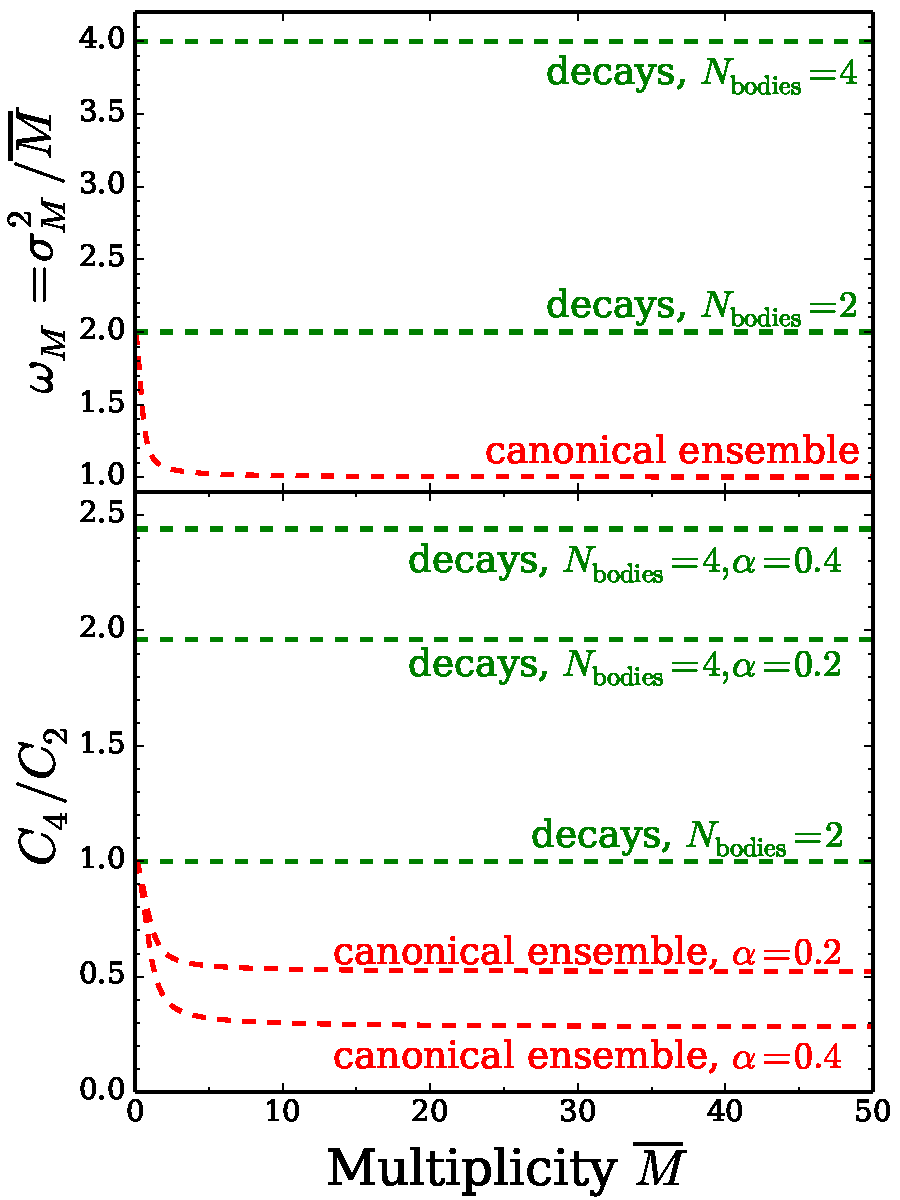
\includegraphics[width=0.5\textwidth]{figs/savchuck}}
\caption{\label{fig:savchuck}
The relative variance of the charged multiplicity distribution is shown for three cases in the upper panel for a system carrying only a single type of unit $\pm$unit charge. For a neutral equilibrated system $\omega$ approaches the Poissonian limit for higher mean multiplicities, $\overline{M}$. This contrasts to a system where one has a Poissonian distribution of neutral particles which all decay into pairs. In this case $\omega=2$ and if the number of charged particles coming from the decay, $N_{\rm bodies}$, of the neutral decay were $n$, one would have $\omega=n$. Using Eq. (\ref{eq:savchuck}) from \cite{savchuck} the ratio $C_4/C_2$ is plotted for the cases above for different fixed efficiencies $\alpha$. For $\omega<2$, $C_4/C_2$ falls below unity, and for $\omega>2$ the ratio exceeds unity. The difference from unity is strongest for $\alpha$ near $1/2$, and the result is symmetric for reflecting $\alpha$ about $1/2$. For $\alpha$ approaching zero or unity $C_4/C_2\rightarrow 1$.}
\end{figure}

\subsection{Decays}

In addition to the results from the canonical ensemble, a system of uncorrelated neutral particles that decays to charged particles is also presented to illustrate the difference in how charge conservation manifests itself in fluctuation observables depending on whether the charges arise directly from an equilibrated system, or whether they arise from the decays of uncorrelated neutral particles. Here, the multiplicity of the uncorrelated neutral particles is assumed to be Poissonian. If each neutral particle decays into $N_{\rm bodies}$ charged particles, where the charges are $\pm 1$, the charged particle multiplicity distributions become 
\begin{eqnarray}
\langle M_{\rm ch}\rangle&=&N_{\rm bodies}\overline{M}_0,\\
\nonumber
\langle(M_{\rm ch}-\overline{M}_{\rm ch})^2\rangle&=&N_{\rm bodies}\langle(M_0-\overline{M}_0)^2\rangle,\\
\nonumber
\omega_M&=&\frac{\langle(M_{\rm ch}-\overline{M}_{\rm ch})^2\rangle}{\overline{M}_{\rm ch}}\\
\nonumber
&=&N_{\rm bodies}\frac{\langle(M_0-\overline{M}_0)^2\rangle}{\overline{M}_0}.
\end{eqnarray}
Fig. \ref{fig:savchuck} illustrates how this picture affects $C_4/C_2$. In this case, because $\omega$ depends only on $N_{\rm bodies}$ and does not change with multiplicity or system size, the cumulants are also independent of multiplicity. For $N_{\rm bodies}=2$ the cumulant ratios does not even depend on the efficiency. For $N_{\rm bodies}>2$ the ratio $C_4/C_2$ exceeds unity, so if charge creation proceeded through the creation and decay of neutral clusters it would be easy to generate large values of $C_4/C_2$. This has been discussed at length in \cite{Bzdak:2018uhv}.

In an equilibrated system decays and recombination have equal rates. However, as the system decouples recombination stops and decays proceed until only stable hadrons remain. Very few decays proceed via more than on charged pair. During the hadronic phase the number of charged particles nearly doubles due to these decays. Thus, if the systems do equilibrate, then decay after chemical freeze-out, one would expect the ratio $C_4/C_2$ to lie somewhere between the value for the canonical ensemble in Fig. \ref{fig:savchuck} and the value for pure decays with $N_{\rm bodies}=2$. STAR's experimental results for net proton fluctuations indeed satisfy this expectation, but their measured $C_4/C_2$ for net charge fluctuations well exceed unity. This discrepancy could be due to volume fluctuations or the decay of larger clusters, or perhaps some shortcoming in this overly simple picture, e.g. the neglect of other conservation laws or Bose condensation. 

\subsection{Bose correlations}

It has long been understood that Bose correlations induce super-Poissonian fluctuations. Here, we illustrate how Bose effects combine with charge conservation to determine $C_4/C_2$. Partition functions for a gas of positive and negative pions, $m_\pi=139.57$ MeV/$c^2$, were considered to be kinetically equilibrated but with a chemical potential enforcing a fixed average density. If a gas is created at chemical equilibrium one expects $\mu=0$, but if it cools while maintaining a fixed number of pions, and if the pion number is fed by decays, a non-zero value of $\mu$ is required. At decoupling one expects kinetic temperatures to fall near 100 MeV and the pion chemical potential to grow to perhaps as high as 75 MeV \cite{Greiner:1993jn}. This estimate can be understood by the fact that the phase space occupancies should stay roughly constant for fixed entropy per particle for an expansiony at fixed entropy, which suggests a chemical potential of approximately 50 MeV by the time the system cools to 100 MeV. Decay products can then further feed the phase space occupancy. Pion condensation occurs when this chemical potential reaches the pion mass. In the absence of Bose effects, this requires roughly doubling the phase space density of pions as compared to the expectations above. If such conditions were realized Bose effects could result in super-radiance \cite{}, which should be accompanied by large multiplicity fluctuations. 

\begin{figure}
\centerline{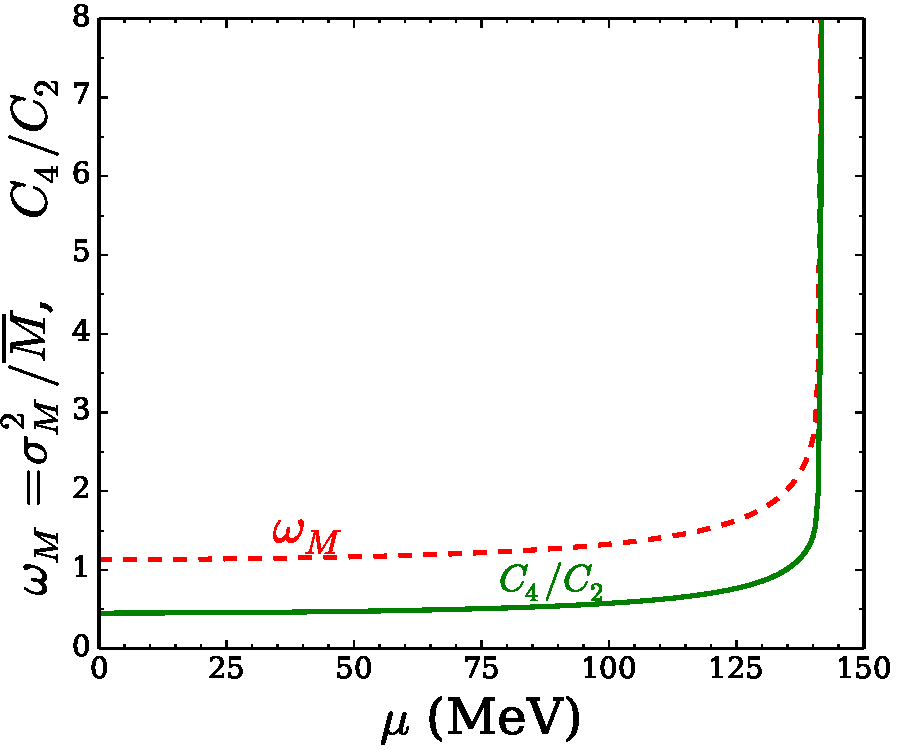
\includegraphics[width=0.4\textwidth]{figs/C4_bose}}
\caption{\label{fig:cheapbose}
Fluctuations for a canonical ensemble at fixed charge, $Q=0$, with an effective chemical potential, $\mu$, applied to adjust the net pion number in a volume of 500 fm$^3$ at a temperature of 100 MeV. The relative variance of the multiplicity distribution (dashed red line) and the ratio $C_4/C_2$ of the net-charge distribution (solid green line) grow dramatically as $\mu$ approaches the pion mass. Super-radiant effects can take place once $\mu$ reaches $m_\pi=139.57$ MeV. Heavy-ion collisions are expected to decouple with effective chemical potentials near 75 MeV, which is well below the onset of large fluctuations.
}
\end{figure}
As a function of the effective chemical potential $\mu$, the partition function for a pion gas in a volume of 500 fm$^3$ and at a temperature of 100 MeV was calculated from Eq. (\ref{eq:Zbf}). For $\mu$ in the range of of 75 MeV the relative variance of the charged multiplicity distribution is $\omega_M\approx 1.2$, which modestly increase $C_4/C_2$ as shown in Fig. \ref{fig:cheapbose} for a fixed efficiency of $\alpha=0.3$. More dramatic results for $C_4/C_2$ are not expected unless the chemical potential would get within a few MeV of the pion mass. As discussed above, this is not expected. However, if the number of pion sources fluctuated wildly from one event to another, and if there were some events with twice the number of sources emitting into the same phase space, super-radiance might occur in some small fraction of the events. Such behavior would strongly contradict expectations based on chemical equilibrium. 


\subsection{Hadron Gas}\label{sec:hadrongas_cheap}

Thus far, all the simple examples presented in this section considered a system with one type of conserved charge, whereas a hadron gas obeys the conservation of baryon number, strangeness and electric charge. This invalidates the use of the recurrence relation of Eq. (\ref{eq:savchuck}) and requires the application of Eq. (\ref{eq:recurrence}), or if Bose corrections are included, Eq. (\ref{eq:bose}). Here, we calculate the canonical ensemble, $Z_A(Q,B,S)$, using the recurrence relation, then apply the Monte Carlo techniques of Sec. \ref{sec:theoryMC} to generate sample sets of particles. The calculation is based on a large number, $\sim 300$, hadron resonances listed in \cite{Tanabashi:2018oca}. After generating the particles, unstable resonances are decayed. For this section, a uniform efficiency $\alpha$ is assumed, independent of species, momenta, or whether the products came from a weak decay (charged pions and kaons were not decayed).

Emission is assumed to come from sub-volumes, or patches, of fixed size. Because each volume is independent, there are no correlations between the various sub-volumes and because cumulants scale linearly with the number of sub-volumes, the ratios of cumulants depend only on the patch volume, not on the overall volume. However, if the number of patches fluctuates, the result would be modified by volume fluctuations. One would expect similar modifications as shown in Sec. \ref{sec:volumefluc}.

Here, the sensitivity to three parameters is investigated. The three parameters are the patch volume, the baryon density, and the fixed efficiency. When one parameter is varied, the other two are set at default values. The default calculation is that the temperature is set at $T=150$ MeV, the baryon density is set to $\rho_B=0$, the efficiency is $\alpha=0.3$ and the default patch volume is 200 fm$^3$. The net electric charge is set to by 0.4 times the average baryon density. After these sensitivities are studied, a calculation at finite baryon density is modified so that the net baryon charge responsible for the non-zero charge density is allowed to fluctuate according to a Poissonian distribution. This is motivated by the fact that the non-zero baryon density comes from charges transported far away from mid-rapidity at early times, so that local charge conservation should play little role for its distribution.

First, the dependence on patch size is exhibited in  Fig. \ref{fig:simple_patchsize}. For small patches the emission of baryons is discouraged because each baryon must be accompanied by the existence of an anti-baryon. Thus, the Boltzmann factor, $e^{-M/T}$, for the mass is compounded by the existence of a second....

% RACHEL -- make figures for
% Default T=150 MeV, Patch Volume=200 fm^3, alpha=0.3
% A. C_4/C_2 for net protons and for net charge with default+ rho_B=0 vs Volume
% B. C_4/C_2 for net protons and for net charge with default+ rho_B=0 vs alpha
% C. C_4/C_2 and C_3/C_1 for net protons and for net charge for default vs rho_B=0={0,0.02,0.04,0.06..., 0.3} with fixed charge
% D. Same as (C) but with "fixed" charge fluctuating according to Poisson about average
%
